% Detailed layer-level architecture of the Stage-1 regression network
% StormCastUNet F_theta (frozen while training MF_theta). All module names,
% channel transitions and parameter counts are measured by instantiating the
% canonical 192x96 network (stormcast/meanflow_architecture.md, "Full layer
% inventory"). Symbols follow the meancasthd.png schematic: M_t, S_t, I,
% F_theta, mu_{t+1}.
\documentclass[border=12pt]{standalone}
% Shared style for the MeanFlow thesis figures.
% Clean academic grayscale, in the spirit of the nntikz examples
% (rounded gray!10 blocks, -latex arrows). Self-contained: this does NOT
% depend on the legacy presentation/meanflow_workflow/src/mf_style.tex.
\usepackage{amsmath,amssymb,bm}
\usepackage{tikz}
\usetikzlibrary{positioning,arrows.meta,calc,fit,backgrounds,shapes.geometric,chains,decorations.pathmorphing}

\tikzset{
  % --- generic nodes ---------------------------------------------------
  base/.style    ={rounded corners=2.5pt, draw, line width=0.8pt, align=center,
                   inner sep=5pt, font=\small, text=black!88},
  block/.style   ={base, fill=gray!10},
  data/.style    ={base, fill=white},                       % data / tensors
  net/.style     ={base, fill=gray!22, line width=1.0pt},   % trained network
  frozen/.style  ={base, fill=gray!4, draw=black!60,        % frozen network
                   dash pattern=on 3pt off 2pt},
  loss/.style    ={base, fill=gray!10, line width=1.0pt,    % loss / scalar
                   double, double distance=1.2pt},
  emph/.style    ={base, fill=gray!10, line width=1.3pt},   % highlighted box
  % --- operator glyphs -------------------------------------------------
  op/.style      ={circle, draw, line width=0.8pt, fill=white,
                   minimum size=4.6mm, inner sep=0, font=\footnotesize},
  concat/.style  ={rectangle, rounded corners=1pt, draw, fill=black!72,
                   text=white, font=\scriptsize\bfseries, inner sep=2.5pt},
  % --- arrows ----------------------------------------------------------
  arrow/.style   ={-{Latex[length=2.4mm]}, line width=0.8pt, draw=black!82},
  arrowc/.style  ={arrow, rounded corners=3pt},
  thinarrow/.style={-{Latex[length=2.0mm]}, line width=0.6pt, draw=black!55},
  loopback/.style={-{Latex[length=2.4mm]}, line width=0.8pt, draw=black!55,
                   dashed, dash pattern=on 4pt off 3pt},
  % --- containers / annotation ----------------------------------------
  group/.style   ={rounded corners=5pt, draw=black!40, line width=0.7pt,
                   dashed, dash pattern=on 3pt off 2.5pt, fill=black!2,
                   inner sep=8pt},
  ttl/.style     ={font=\bfseries\large, text=black!88},
  sub/.style     ={font=\itshape\footnotesize, text=black!55},
  lab/.style     ={font=\scriptsize, text=black!70},
  tag/.style     ={font=\scriptsize\bfseries, text=black!60},
  % small sine glyph used to mark Fourier / positional embeddings
  sinewave/.style={decorate, decoration={snake, amplitude=0.6mm,
                   segment length=2.2mm}},
}

% legend swatch helper: \swatch{<style>}{<label>}
\newcommand{\swatch}[2]{%
  \tikz[baseline=-0.5ex]\node[#1, minimum width=3.6mm, minimum height=2.8mm,
    inner sep=0]{};\;#2}

\begin{document}
\newcommand{\restag}[1]{{\tiny\bfseries\textcolor{black!55}{#1}}}
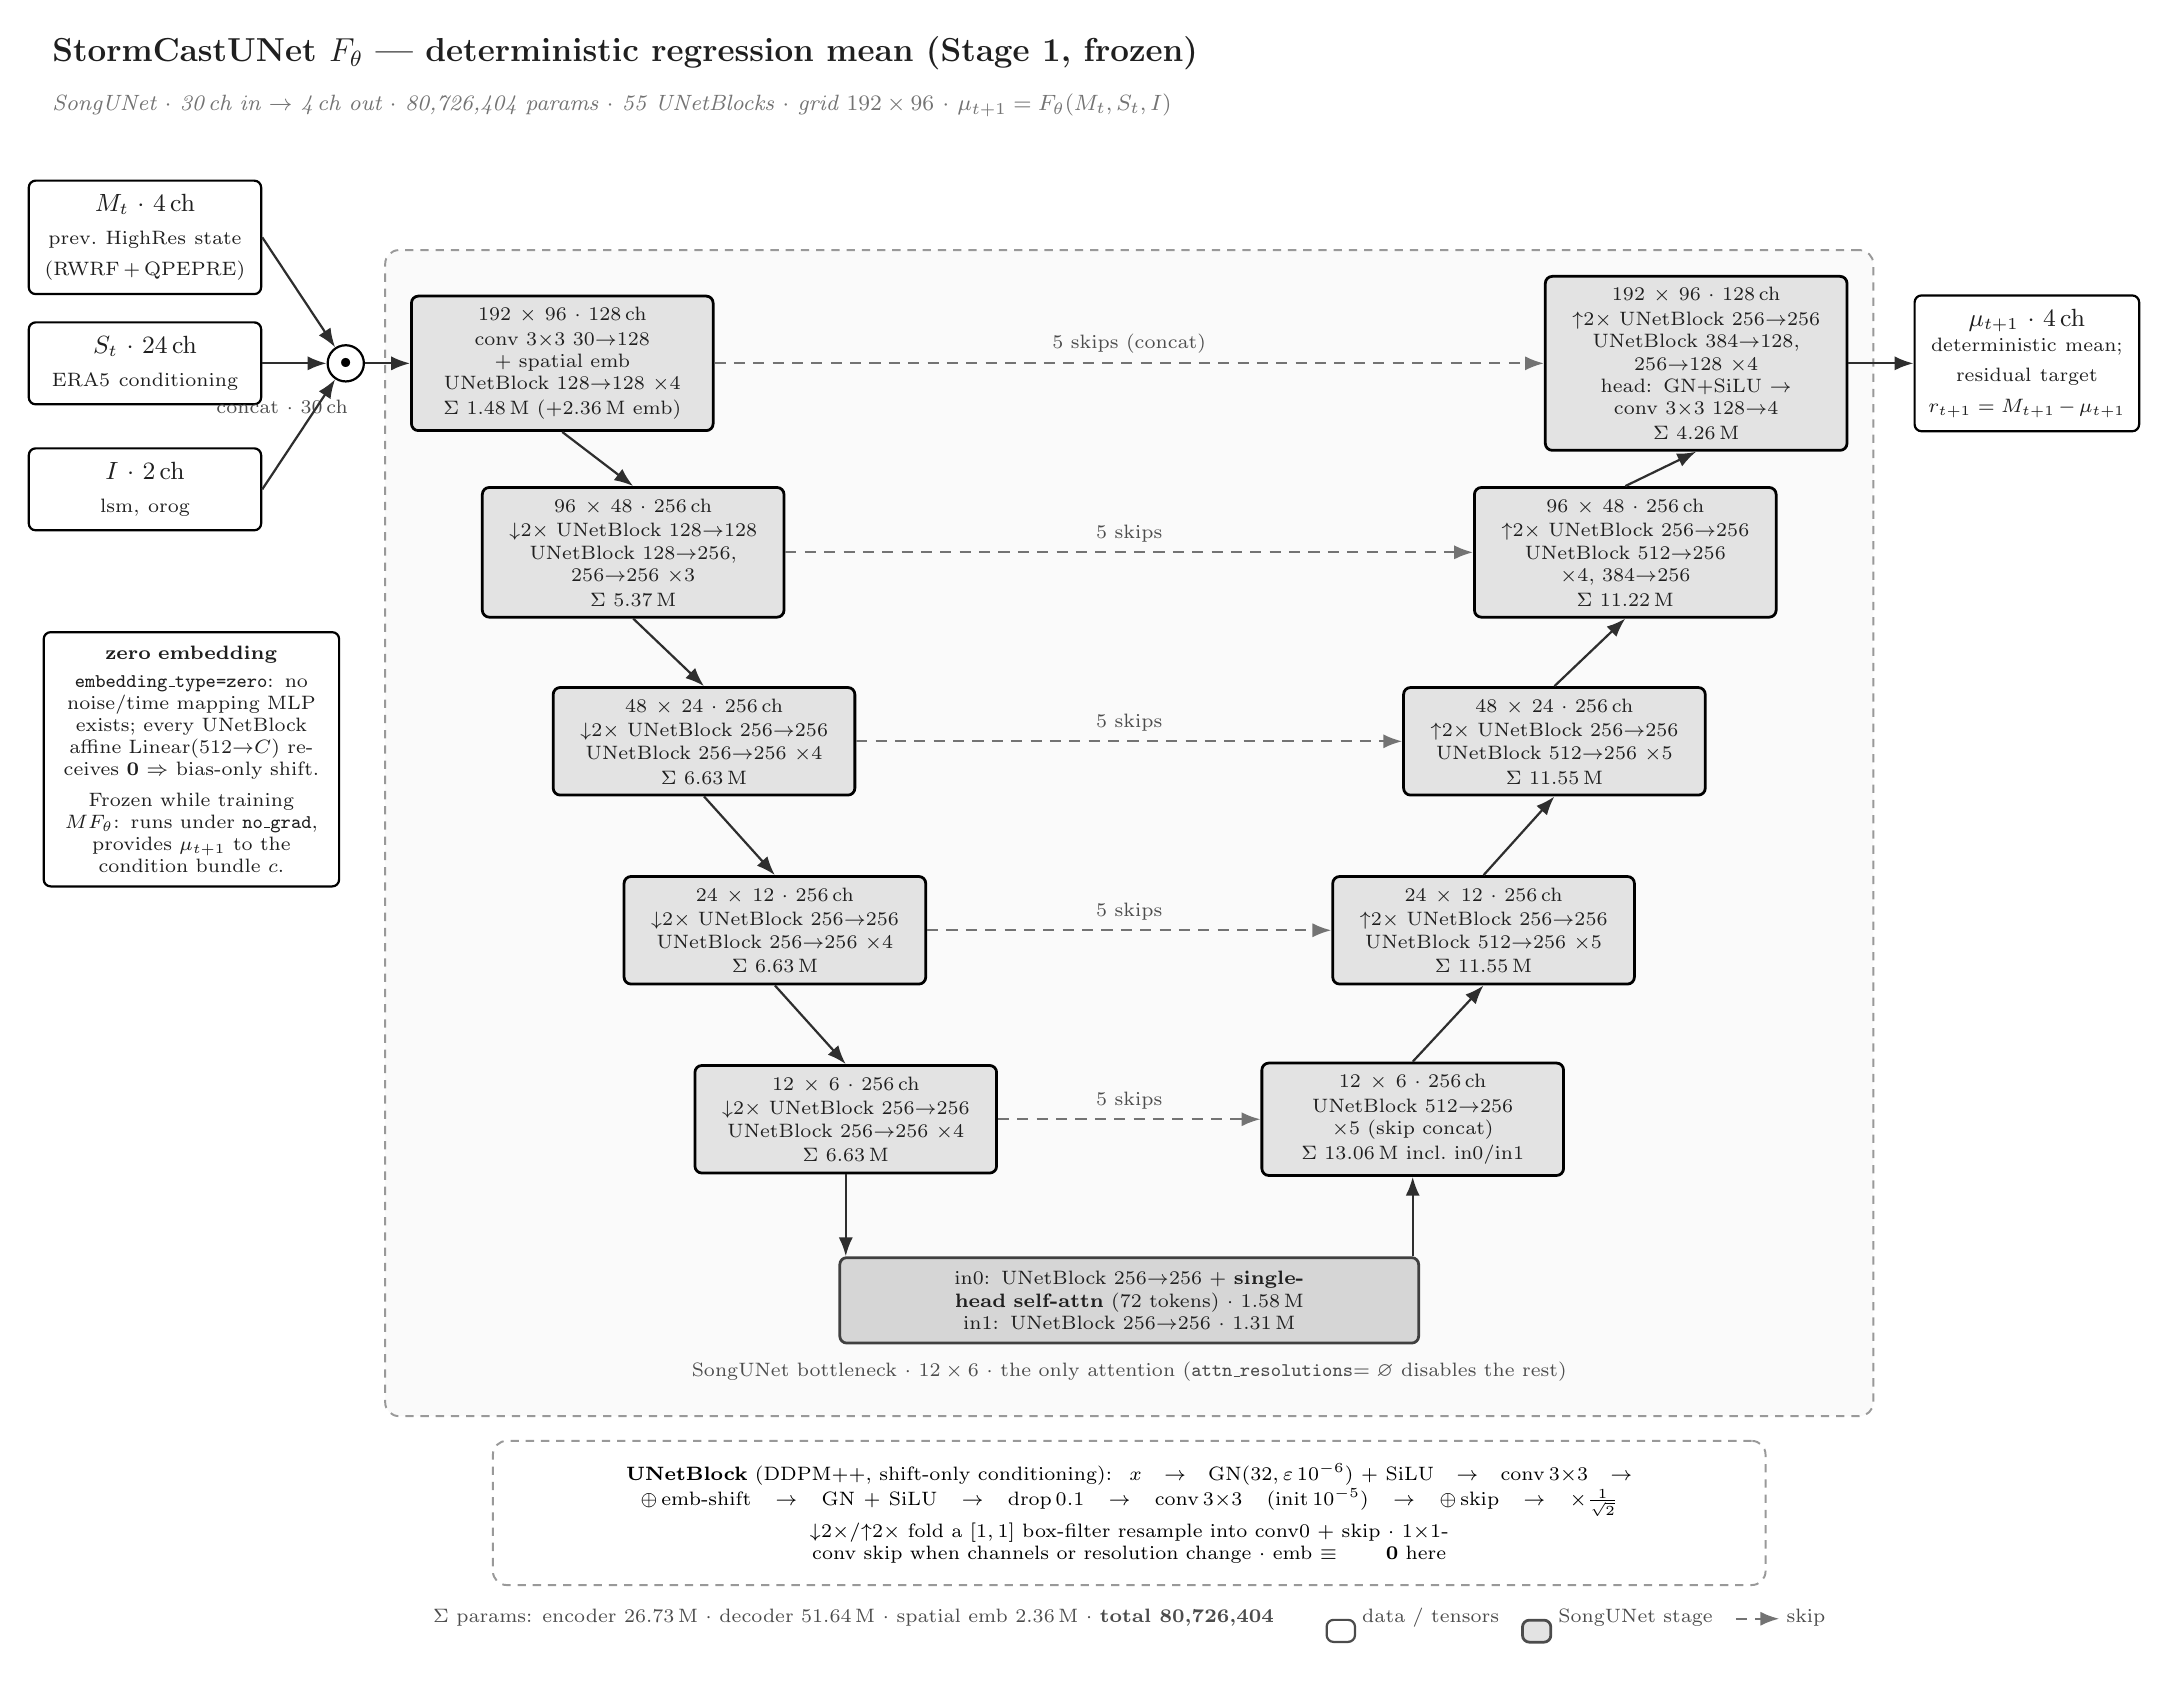
\begin{tikzpicture}
  % stage box style for the U levels
  \tikzset{ustage/.style={net, text width=3.55cm, font=\scriptsize, inner sep=4pt}}

  % ============================ inputs + concat ============================
  \node[data, text width=2.6cm] (mt) at (-5.3, 1.6)
    {$M_t$ $\cdot$ 4\,ch\\[1pt]\scriptsize prev.\ HighRes state (RWRF\,+\,QPEPRE)};
  \node[data, text width=2.6cm] (st) at (-5.3, 0.0)
    {$S_t$ $\cdot$ 24\,ch\\[1pt]\scriptsize ERA5 conditioning};
  \node[data, text width=2.6cm] (iv) at (-5.3,-1.6)
    {$I$ $\cdot$ 2\,ch\\[1pt]\scriptsize lsm, orog};
  \node[op] (cc) at (-2.75, 0) {$\bullet$};
  \node[lab, anchor=north east] at ($(cc.south)+(1.5mm,-1mm)$) {concat $\cdot$ 30\,ch};

  \draw[arrow] (mt.east) -- (cc);
  \draw[arrow] (st.east) -- (cc);
  \draw[arrow] (iv.east) -- (cc);

  % ============================ encoder (staircase down-right) ============================
  \node[ustage] (e0) at (0.0, 0.0) {%
    \restag{$192\times96$ $\cdot$ 128\,ch}\\[1pt]
    conv $3{\times}3$ $30{\to}128$ $+$ spatial emb\\
    UNetBlock $128{\to}128$ $\times4$\\[1pt]
    $\Sigma$ 1.48\,M ($+$2.36\,M emb)};
  \node[ustage] (e1) at (0.9,-2.4) {%
    \restag{$96\times48$ $\cdot$ 256\,ch}\\[1pt]
    ${\downarrow}2{\times}$ UNetBlock $128{\to}128$\\
    UNetBlock $128{\to}256$, $256{\to}256$ $\times3$\\[1pt]
    $\Sigma$ 5.37\,M};
  \node[ustage] (e2) at (1.8,-4.8) {%
    \restag{$48\times24$ $\cdot$ 256\,ch}\\[1pt]
    ${\downarrow}2{\times}$ UNetBlock $256{\to}256$\\
    UNetBlock $256{\to}256$ $\times4$\\[1pt]
    $\Sigma$ 6.63\,M};
  \node[ustage] (e3) at (2.7,-7.2) {%
    \restag{$24\times12$ $\cdot$ 256\,ch}\\[1pt]
    ${\downarrow}2{\times}$ UNetBlock $256{\to}256$\\
    UNetBlock $256{\to}256$ $\times4$\\[1pt]
    $\Sigma$ 6.63\,M};
  \node[ustage] (e4) at (3.6,-9.6) {%
    \restag{$12\times6$ $\cdot$ 256\,ch}\\[1pt]
    ${\downarrow}2{\times}$ UNetBlock $256{\to}256$\\
    UNetBlock $256{\to}256$ $\times4$\\[1pt]
    $\Sigma$ 6.63\,M};

  % ============================ decoder (staircase up-right) ============================
  \node[ustage] (d4) at (10.8,-9.6) {%
    \restag{$12\times6$ $\cdot$ 256\,ch}\\[1pt]
    UNetBlock $512{\to}256$ $\times5$ (skip concat)\\[1pt]
    $\Sigma$ 13.06\,M incl.\ in0/in1};
  \node[ustage] (d3) at (11.7,-7.2) {%
    \restag{$24\times12$ $\cdot$ 256\,ch}\\[1pt]
    ${\uparrow}2{\times}$ UNetBlock $256{\to}256$\\
    UNetBlock $512{\to}256$ $\times5$\\[1pt]
    $\Sigma$ 11.55\,M};
  \node[ustage] (d2) at (12.6,-4.8) {%
    \restag{$48\times24$ $\cdot$ 256\,ch}\\[1pt]
    ${\uparrow}2{\times}$ UNetBlock $256{\to}256$\\
    UNetBlock $512{\to}256$ $\times5$\\[1pt]
    $\Sigma$ 11.55\,M};
  \node[ustage] (d1) at (13.5,-2.4) {%
    \restag{$96\times48$ $\cdot$ 256\,ch}\\[1pt]
    ${\uparrow}2{\times}$ UNetBlock $256{\to}256$\\
    UNetBlock $512{\to}256$ $\times4$, $384{\to}256$\\[1pt]
    $\Sigma$ 11.22\,M};
  \node[ustage] (d0) at (14.4, 0.0) {%
    \restag{$192\times96$ $\cdot$ 128\,ch}\\[1pt]
    ${\uparrow}2{\times}$ UNetBlock $256{\to}256$\\
    UNetBlock $384{\to}128$, $256{\to}128$ $\times4$\\
    head: GN$+$SiLU $\to$ conv $3{\times}3$ $128{\to}4$\\[1pt]
    $\Sigma$ 4.26\,M};

  % ============================ bottleneck ============================
  \node[net, fill=gray!32, draw=black!75, text width=7.0cm, font=\scriptsize]
    (bk) at (7.2,-11.9)
    {in0: UNetBlock $256{\to}256$ $+$ \textbf{single-head self-attn} (72 tokens) $\cdot$ 1.58\,M\\
     in1: UNetBlock $256{\to}256$ $\cdot$ 1.31\,M};
  \node[lab, anchor=north] (bkcap) at ($(bk.south)+(0,-1mm)$)
    {SongUNet bottleneck $\cdot$ $12\times6$ $\cdot$ the only attention
     (\texttt{attn\_resolutions}$=\varnothing$ disables the rest)};

  % ============================ U-Net container ============================
  \begin{scope}[on background layer]
    \node[group, fit=(e0)(e4)(bk)(bkcap)(d4)(d0), inner sep=9pt] (unet) {};
  \end{scope}

  % ============================ main data path ============================
  \draw[arrow] (cc) -- (e0.west);
  \draw[arrow] (e0.south) -- (e1.north);
  \draw[arrow] (e1.south) -- (e2.north);
  \draw[arrow] (e2.south) -- (e3.north);
  \draw[arrow] (e3.south) -- (e4.north);
  \draw[arrow] (e4.south) -- ($(bk.north -| e4.south)$);
  \draw[arrow] ($(bk.north -| d4.south)$) -- (d4.south);
  \draw[arrow] (d4.north) -- (d3.south);
  \draw[arrow] (d3.north) -- (d2.south);
  \draw[arrow] (d2.north) -- (d1.south);
  \draw[arrow] (d1.north) -- (d0.south);

  % ============================ skip connections ============================
  \draw[loopback] (e0.east) -- node[lab,above,pos=0.5]{5 skips (concat)} (d0.west);
  \draw[loopback] (e1.east) -- node[lab,above,pos=0.5]{5 skips} (d1.west);
  \draw[loopback] (e2.east) -- node[lab,above,pos=0.5]{5 skips} (d2.west);
  \draw[loopback] (e3.east) -- node[lab,above,pos=0.5]{5 skips} (d3.west);
  \draw[loopback] (e4.east) -- node[lab,above,pos=0.5]{5 skips} (d4.west);

  % ============================ output ============================
  \node[data, text width=2.5cm] (out) at (18.6, 0.0)
    {$\mu_{t+1}$ $\cdot$ 4\,ch\\[1pt]\scriptsize deterministic mean;\\
     residual target $r_{t+1} = M_{t+1} - \mu_{t+1}$};
  \draw[arrow] (d0.east) -- (out.west);

  % ============================ specifics note ============================
  \node[data, text width=3.4cm, font=\scriptsize, anchor=north west]
    (note) at (-6.6,-3.4)
    {\textbf{zero embedding}\\[2pt]
     \texttt{embedding\_type=zero}: no noise/time mapping MLP exists;
     every UNetBlock affine $\mathrm{Linear}(512{\to}C)$ receives $\bm{0}$
     $\Rightarrow$ bias-only shift.\\[3pt]
     Frozen while training $MF_\theta$: runs under \texttt{no\_grad},
     provides $\mu_{t+1}$ to the condition bundle $c$.};

  % ============================ title ============================
  \node[ttl, anchor=south west] (title) at (-6.6, 3.6)
    {StormCastUNet $F_\theta$ --- deterministic regression mean (Stage 1, frozen)};
  \node[sub, anchor=north west] at ($(title.south west)+(0,-0.6mm)$)
    {SongUNet $\cdot$ 30\,ch in $\to$ 4\,ch out $\cdot$ 80{,}726{,}404 params
     $\cdot$ 55 UNetBlocks $\cdot$ grid $192\times96$ $\cdot$
     $\mu_{t+1} = F_\theta(M_t, S_t, I)$};

  % ============================ UNetBlock anatomy + totals ============================
  \node[group, text width=15.6cm, font=\scriptsize, align=center, fill=white]
    (anatomy) at (7.2,-14.6)
    {\textbf{UNetBlock} (DDPM++, shift-only conditioning):\;
     $x \to \mathrm{GN}(32,\varepsilon\,10^{-6})\!+\!\mathrm{SiLU}
     \to \mathrm{conv}\,3{\times}3 \to \oplus\,\text{emb-shift}
     \to \mathrm{GN}\!+\!\mathrm{SiLU} \to \mathrm{drop}\,0.1
     \to \mathrm{conv}\,3{\times}3\;(\text{init}\,10^{-5})
     \to \oplus\,\text{skip} \to \times\tfrac{1}{\sqrt{2}}$\\[1pt]
     ${\downarrow}2{\times}/{\uparrow}2{\times}$ fold a $[1,1]$ box-filter resample
     into conv0 $+$ skip $\cdot$ 1$\times$1-conv skip when channels or
     resolution change $\cdot$ emb $\equiv \bm{0}$ here};
  \node[lab, anchor=north] at ($(anatomy.south)+(0,-1.6mm)$)
    {$\Sigma$ params: encoder 26.73\,M $\cdot$ decoder 51.64\,M $\cdot$
     spatial emb 2.36\,M $\cdot$ \textbf{total 80{,}726{,}404} \qquad
     \swatch{data}{data / tensors}\quad
     \swatch{net}{SongUNet stage}\quad
     \tikz[baseline=-0.5ex]\draw[loopback](0,0)--(0.55,0);\;skip};

\end{tikzpicture}
\end{document}
